\chapter{Introdução}
\par A eclosão da pandemia do coronavírus tem se mostrado o maior choque enfrentado pela economia brasileira em anos recentes, tanto pela lado da demanda com a contração do consumo das famílias e dos investimentos, quanto pelo lado da oferta, com a interrupção temporária de atividades produtivas ou mesmo pela falência de empresas.

Soma-se a isso a fragilidade fiscal do Estado brasileiro e o alto nível de desemprego que já estava em níveis altos desde a recessão de 2015/2016. Tudo isso faz com que possamos esperar um cenário preocupante para a economia brasileira como um todo.


\par Nesse sentido, podemos esperar também um grande choque na economia tocantinense. Os indicadores que serão apresentados ao longo das seções deste Boletim farão um retrato de como esse grande choque afetou e poderá afetar a economia do nosso estado.
\begin{smbox}[label={labelbox},nameref={Cálculo do PIB e as suas óticas}]{Cálculo do PIB e as suas óticas}
	O Produto Interno Bruto (PIB) é a soma de todos os bens e serviços finais produzidos por um país. É possível calcula-lo pela ótica da oferta, somando tudo aquilo que é produzido por todos os setores, pela ótica da demanda, somando o consumo das famílias, consumo do governo, investimentos e exportações liquidas (exportações menos importações) e também pela ótica da renda, somando toda renda da população. O resultado das três óticas é sempre o mesmo.
\end{smbox}
\par No primeiro trimestre e no segundo semestre de 2020 o PIB brasileiro encolheu 2,5\% e 9,7\%, respectivamente. Esses resultados foram os primeiros sinais dos efeitos da pandemia da COVID-19, sendo que seu resultado negativo em partes explicados pelas medidas de fechamento de comércios e serviços a fim de evitar a propagação do vírus, sobretudo no segundo semestre.

\begin{figure}[ht]
	\caption{Variação trimestral do PIB com ajuste sazonal}
	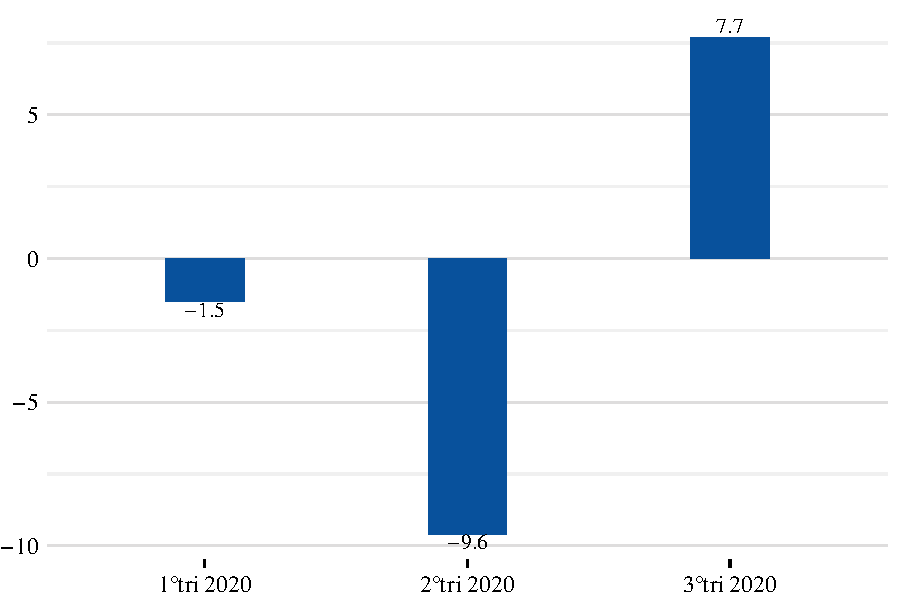
\includegraphics[width=\linewidth]{fig/pib_total.pdf}
	\source{IBGE}
	\notes{Elaboração própria}
\end{figure}
\par Se olharmos o lado da demanda é possível ver uma queda generalizada sobre todos os componentes, com exceção das Exportações. Mesmo os Investimentos, que no primeiro semestre ainda registrava alta de 2,3\% teve a maior queda do segundo semestre com um recuo de 15,4\%.
\begin{figure}[ht]
	\caption{Variação trimestral do PIB pelo lado da demanda}
	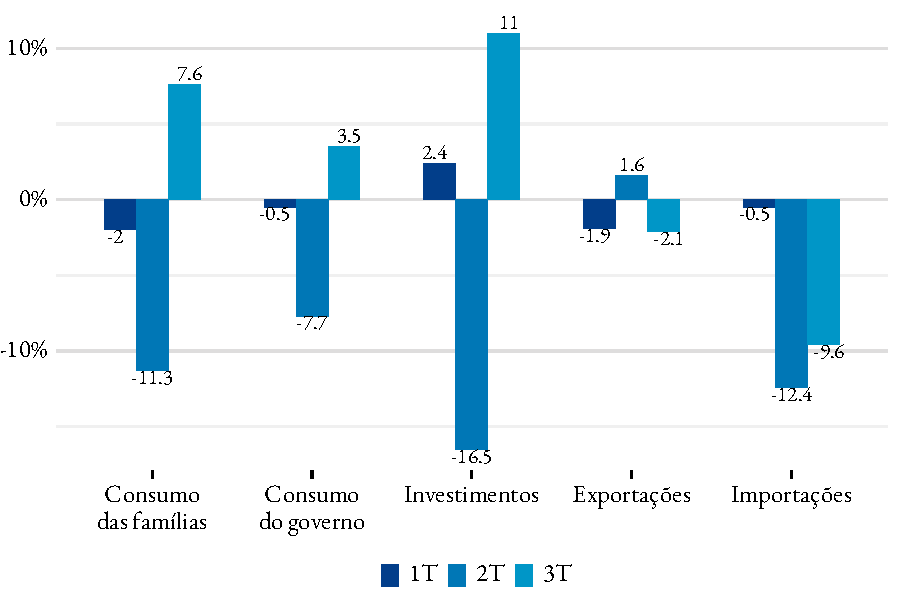
\includegraphics[width=\linewidth]{fig/pib_demanda.pdf}
	\source{IBGE}
	\notes{Elaboração própria}
\end{figure}
\par Pelo lado da oferta o único setor com resultado positivo foi o agropecuário, setor menos afetado pelas medidas de isolamento, e o que em parte explica o bom desempenho das exportações no lado da demanda, com sua altas de 0,5\% e 0,4\%. No setor de serviços, que representa nada menos do que 72\% do nosso PIB, as quedas de 2,2\% e 9,7\% pesaram bastante para a queda total. Já as quedas de 0,8\% e 12,3\% da indústria perpetuam ainda mais o encolhimento desse setor dentro da economia brasileira.
\begin{figure}[ht]
	\caption{Variação trimestral do PIB pelo lado da oferta}
	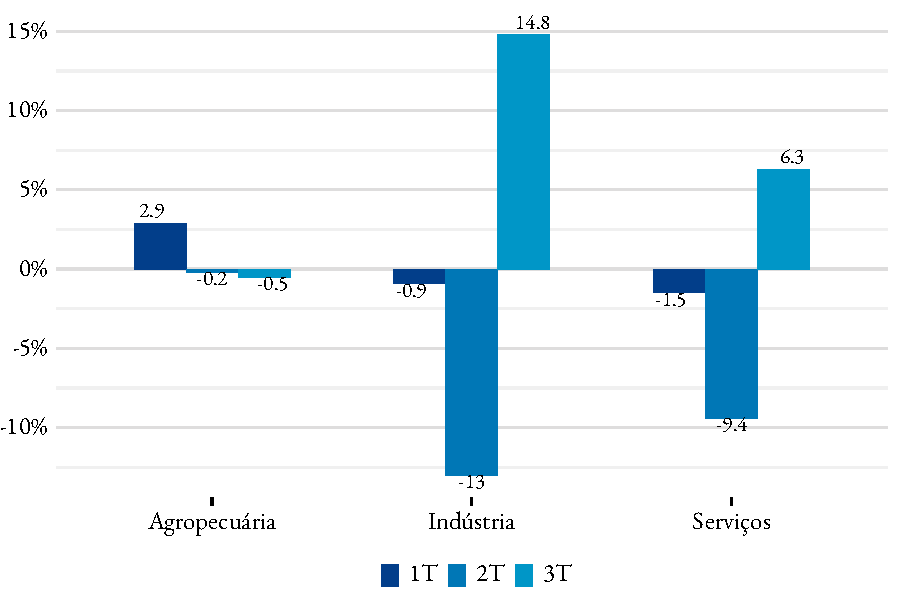
\includegraphics[width=\linewidth]{fig/pib_oferta.pdf}
	\source{IBGE}
	\notes{Elaboração própria}
\end{figure}
\par Nesse sentido, se coloca um grande desafio para economia tocantinense que é o de superar esse grande choque nunca antes visto na história do do nosso jovem estado. Como já mencionado, é esperado que todas as variáveis discutidas ao longo deste Boletim sofram um forte impacto, tanto no curto, quanto no longo prazo. Pensar e discutir maneiras de lidar com esse choque adverso é um tema primordial na recuperação pós-pandemia para que a economia do nosso estado possa ter uma boa recuperação e para que se aumente a qualidade de vida do cidadão tocantinense ao longo de todo o estado. 
